\documentclass{article}
\usepackage{amsmath,amsfonts,amsthm,amssymb,wasysym}
\usepackage{setspace}
\usepackage{enumitem}
\usepackage{Tabbing}
\usepackage{fancyhdr}
\usepackage{lastpage}
\usepackage{chngpage}
\usepackage{url}
\usepackage{subfigure}
\usepackage{array}
\usepackage{multicol}
\usepackage[color=blue!40]{todonotes}
\usepackage[protrusion=true,expansion,kerning]{microtype}
\usepackage{natbib}

% to adjust margins:
\topmargin=-0.25in
\evensidemargin=0in
\oddsidemargin=0in
\textwidth=6.25in
\textheight=8.5in
\headsep=0.25in

% homework specific information
\newcommand{\hmwkTitle}{Patent Classification}
\newcommand{\hmwkDueDate}{December 6, 2013}
\newcommand{\hmwkClass}{}
\newcommand{\hmwkClassInstructor}{}
\newcommand{\hmwkAuthorName}{Sullivan, Cellier, Hobbs}

% math aliases
\newcommand{\reals}{\mathbb{R}}
\newcommand{\twopartdef}[4]
{
	\left\{
		\begin{array}{ll}
			#1 & \mbox{if } #2 \\
			#3 & \mbox{if } #4
		\end{array}
	\right.
}

% header and footer
\pagestyle{fancy}
\lhead{\hmwkAuthorName}
\chead{\hmwkTitle}
\rhead{\hmwkDueDate}   
\lfoot{}
\cfoot{}
\rfoot{\emph{Page\ \thepage\ of\ \pageref{LastPage}}}                          
\renewcommand\headrulewidth{0.4pt}
\renewcommand\footrulewidth{0.4pt}

\makeatletter
\newenvironment{tablehere}
  {\def\@captype{table}}
  {}

\newenvironment{figurehere}
  {\def\@captype{figure}}
  {}
\makeatother

%\renewcommand{\bibsection}{\subsubsection*{\refname}}

% Make title 
\title{
\LARGE\bf Patent Classification using Supervised Methods \\
\date{}
\author{ John Sullivan \and Caitlin Cellier \and J. Nicholas Hobbs}
}

\begin{document}

\maketitle

\input{abstract}

\thispagestyle{fancy}

\maketitle

%%%%%%%%%%%%%%%%%%%%%%%%%%%%%%%%%%%%%%%%%%%%%%%%%%%%%%%%%%%%%%%%%
\section{Introduction}
\indent
The United States Patent Office (USPTO) granted 276,788 patents in 2012\cite{USPTO:2013:stats}. This is more than double the number granted 20 years ago, and rate of filings is still increasing. In the circumstance it makes sense to consider scalable, automated approaches to parts of the patent review process. To this end we examined attempting to classify patents into existing categorizations using supervised machine learning techniques. We also attempted to measure the coherency and usefulness of the classifications. Reliable automation of patent categorization is an important first step to larger scale automation of the patent review process.

In this paper we experimented with several machine learning classifiers to automatically categorize patents into each of the 8 top-level patent categories specified in the International Patent Classification\cite{ipc:2013:guide} (IPC). The USPTO is moving from its previous classification system (which contained thousands of classes and was deemed unsuitable for standard machine learning classification techniques) to the Cooperative Patent Classification (CPC), which is a superset of the IPC. The USPTO labels with an IPC Classification in preparation for this conversion. The CPC classification conforms to the IPC classification, but also contains one additional category, Y, which is for patents on technologies that span several sections of the IPC classification. All patents must contain at least one primary classification, but may be assigned more if they are relevant to multiple IPC classes. In our experiments we only attempted to classify the primary classification.


% Relative size of categories?

\begin{tablehere}
	\centering
	\caption{IPC Classifications and their titles}
	\begin{tabular}{ | l | l |}
		\hline
		\textbf{Class} & \textbf{Title} \\
				\hline
		A & Human Necessities \\
				\hline
		B & Performing Operations; Transporting \\
				\hline
		C & Chemistry; Metallurgy \\
				\hline
		D & Textiles; Paper \\
				\hline
		E & Fixed Constructions \\
				\hline
		F & Mechanical Engineering; Lighting; Heating; Weapons; Blasting Engines or Pumps \\
		\hline
		G & Physics \\
				\hline
		H & Electricity \\
				\hline
	\end{tabular}
	
\end{tablehere}



%Many of these patents are awarded to so-called nonpracticing entities (NPEs), organizations that do not design, build (or even prototype) the techniques and technologies under patent, but rather create or invest in patent portfolios to litigate against organizations or individuals that build related products. At the same time, patent litigation has been increasing, particularly litigation initiated by NPEs\cite[p. 7]{PWC:2013:lit}. In such an environment, it is more important than ever to be able to quickly and reliably assess the quality of patents, both in terms of their content, and whether they represent truly original work. 

% More Here!!

%The structure of the brain influences availability and access to the memories stored therein. Communication between neurons allows animals to think, move, and store or recall memories. It seems plausible that the structure of an artificial neural network would similarly affect the ability of that neural network to store and process information. Building off this idea, we suggest a new model of neural network influenced by Perin, Berger, and Markram (2011) who proposed that the brain is composed of a hierarchy of connected components with specific associated computational functions. 

%We implemented this model within the framework of deep learning inspired by Hinton (2007).  More specifically, we describe a model of deep learning based on the use of acyclic clusters which mimic multiple layers of neurons. Additionally, these clusters themselves are layered. We found that this model did not significantly increase the ability of our network to generate or classify handwritten digits, nor did it increase the computational efficiency of those tasks.
%\label{sec:Introduction}
%%%%%%%%%%%%%%%%%%%%%%%%%%%%%%%%%%%%%%%%%%%%%%%%%%%%%%%%%%%%%%%%%

%Some text, cite this~\cite{ASBMI,Acharya07}, and also Figure~\ref{fig:something}.
\section{Data Set and Feature Selection}
%\cite*{mimno-mccallum-11}

\subsection{Dataset Construction}
\indent
The United States Patent Office makes bulk patent grant information available through several private companies\cite{USPTO:2013:patent-catalog} in XML format\cite{USPTO:2013:dtd}. For our experiments we drew samples from patent grants made between May 1st 2012 and July 31st 2012. Over these three months the USPTO granted a total of 76,317 patents, or roughly 6,000 per week. We constructed three datasets from this, \emph{even-3500}, \emph{jagged-20000}, and \emph{jagged-40000}. \emph{even-3500} consisted of 350 training and 150 test instances from 7 of the 8 IPC patent classes (one class, D, which corresponds to textiles and paper could not be used since a only 47 patents were granted to that section in our dataset). \emph{jagged-20000} and \emph{jagged-40000} were simply a random sample of 20,000 and 40,000 patents respectively granted within the given timeframe, using all 8 of the IPC patent classes.

\subsection{Feature Selection}
\indent
Patents are semi-structured. That is, rather than simply being free text, there are certain fields that all patent grants are guaranteed to have (as well as other, optional fields). This needs to be taken into consideration when designing features for patent classification. 

Although a domain expert could potentially design features that were powerful, we ended up considering three relatively general feature sets, \emph{description-unigrams}, \emph{abstract-bigrams}, and \emph{tf-idf}. \emph{description-unigrams} consists of unigrams from the main ``description'' field of the patent document, tokenized and with stopwords removed. \emph{abstract-bigrams} consists of unigrams and bigrams from the ``abstract'', ``claims'', and ``title'' fields of the patent. \emph{tf-idf} consists of the tokens (and token-pairs) from \emph{abstract-bigrams} weighted them with a statistic called term frequency inverse document frequency (tf-idf)\cite{manning:2008:IR}. Intuitively, the tf-idf weight of a token (or token bigram) in a document increases as the number of times it occurs in that document increases and decreases as the number of times it appears in every other document increases. This weighting gives us a sense of how characteristic the token (or token bigram) is of each document. Once we calculated tf-idf scores for each document, we truncated the word bags to contain only the 32, 100, and 250 highest weighted features for each patent. We used tools in FACTORIE\cite{mccallum09:factorie:} to tokenize the patents and remove stopwords. We also added domain-specific stopwords based on observations of patent documents. 

Both of these bag of n-grams models can be easily translated into vectors. This allows us to use a variety of standard machine learning multiclass classification techniques. For some set of documents $\mathbf{D}$, let $| \mathbf{V} |$ denote the number of unique n-grams that appear in that set of documents (for a given tokenizer and stopword lexicon). Then we can represent each document $ d \in \mathbf{D}$ by a binary vector $f \in \{0,1\}^{| \mathbf{V} |}$, where $f^d_i = 1$ when $d$ contains the $i$\textsuperscript{th} n-gram in the vocabulary and 0 otherwise. Nominally, these feature vectors are very large ($| \mathbf{V} | > 900000$ for \emph{abstract-bigrams} on \emph{jagged-40000}). Thus we need to represent these vectors sparsely in practice in order to work tractably with them.


%Our data is from the United States Patent and Trademark Office Bulk Downloads located on Google.  The original data file is prepared as an XML file, which we then parse to find a list of words contained within the patent.  Based on the total list of words of all patents in a sample, a feature vector is created such that the feature vector includes a feature for every seen word within the dataset.  A 1 is included for a feature within a feature vector for a patent if the patent contains the word, and a 0 is included for a specific feature if the patent did not include the word.  This bag of words technique was used for all experiments.
\section{Classification Techniques}
%%Just have dataset here instead of a whole separate section? If it's in it's own section then we can give a fuller background on the classes and maybe an explanation of the coherence scores
%\subsection{Data Set}

\subsection{Maximum Entropy} % (fold)
\label{sub:maximum_entropy}

\indent
Maximum entropy models are standard tools in document classification\cite{Nigam99usingmaximum}. A maximum entropy classifier calculates a probability distribution over label classes ($c$) conditioned on the observed feature vector. Usually the predicted class of a feature vector is taken to be the class with the highest probability under a learned parameterization of the distribution. The learning step simply involves estimating the natural parameters of an exponential distribution. Customarily the observed feature vector is binary. Taking $f(c,d)$ to represent the feature vector for a single document ($d$) being assigned to a given class, and $\theta$ to be the weight vector we want to learn, this gives
\begin{align*}
	P(c|f, \theta) = \frac{e^{\theta \cdot f(c, d)}}{\sum_{c'} e^{\theta \cdot f(c',d)}}
\end{align*}

We can estimate the parameters of this distribution easily using standard convex optimization techniques. Since this distribution is a natural formulation of the exponential family, it is the distribution that highest entropy subject to the constraints imposed by the observed feature vectors, hence its name. 

In our case where the feature vector is sparse and of very high dimensionality, it is necessary to regularize the learned weight vector $\theta$. Regularization allows us to avoid issues that arise when learned parameter weights would grow too large or be very small. If a given feature only appears in one class of the training data, an unregularized system will learn an infinite weight on it, since it perfectly predicts that class. Conversely, if a feature is a very weak predictor the regularization will push the weight to zero. This acts effectively as an online dimensionality reduction. As is customary, we used a regularization technique that conceptually corresponds to putting a standard normal prior on the learned weights. For these experiments we used the Maximum Entropy model implemented in FACTORIE, which uses LBFGS\cite{Liu89onthe} to perform the gradient descent necessary to estimate parameters.

% subsection maximum_entropy (end)

\subsection{Multi-class SVM} % (fold)
\label{sub:multiclass_svm}

Given a sequence of training examples $(c, x)$ where $c \in \mathbf{C}$ and $x = f(\cdot, d)$ for each $d \in \mathbf{D}$. We define binary functions $y_c(c
') = \twopartdef{1}{ c' = c}{0}{otherwise}$. For multi-class classification we train $| \mathbf{C} |$ binary classifiers. For each class we train a support vector machine by solving a constrained minimization problem for the weight vector:
\begin{align*}
	\min_{w,\xi} & \left( \frac{1}{2} \| \mathbf{w} \|^2 + C \sum_{i=1}^n \xi_i \right) \\
	\text{subject to} &  \text{ } \forall i, \text{ } y_i(w \cdot x_i - b) > 1 - \xi_i, \text{ } \xi_i > 0
\end{align*}

There are a number of black-box SVM implementations that can efficiently train an SVM with multiple different parameter settings. We used LIBSVM\cite{CC01a} to run our SVM experiments. The implementation uses a sequential minimum optimization technique\cite{Fan05workingset} to efficiently minimize $w$. We used linear kernels for all of our experiments, as they have proven useful for document classification in the past\cite{DBLP:conf/ecml/Joachims98}.


%All of our experiments were run with a linear kernel at the default settings. % WHAT ARE THEY?


% subsection multiclass_svm (end)


%\subsection{Supervised Methods}
%For the first experiment, the dataset was created such that each of the 7 classification categories were evenly represented with 200? samples each.  (Define Training/Testing and re-run experiment)

%Description of SVM -------



%% Tempted to make this it's own section as well
\subsection{Dimensionality Reduction}
There are several informal dimensionality reduction techniques that we have used to compress our very high dimensional space into a slightly smaller space. The removal of stopwords can be seen as a very basic dimensionality reduction. Similarly, tf-idf is an unsupervised dimensionality reduction technique that removes dimensions that are likely to have little predictive power.  
\\
\\In addition to these we attempted to use two more traditional dimensionality techniques, principle component analysis (PCA), and Laplacian eigenmap.  For our purposes, we used a MATLAB script titled mani.m by Todd Wittmann \cite{Wittman}.   Saul, Weinberger, Sha, Ham, and Lee. \cite{saul06spectral} provide an intuitive explanation of PCA that is very useful for understanding it.  They state PCA can be viewed as trying to find a set of features which is able to replicate the original variance structure.  As a note, for PCA, the features are ordered such that the features which maximize the variance are selected first.  Saul et a.\cite{saul06spectral} further state that the Laplacian Eigenmap allows for local mappings between inputs to be maintained.  These intuitive descriptions are useful for understanding the results found in our experimental sections.

%Description of PCA and Laplacian


%For the second experiment, the dataset from experiment one had two different dimensionality reduction techniques used to reduce the dataset.  The two included PCA and a Laplacian Eigenmap.  (Define Training/Testing and re-run experiment)

%\subsection{Boosting Methods}
%For the third experiment, we attempted to determine if more data would noticeably improve the results of the algorithm.  Specifically, the dataset was expanded to approximately 2000 samples each. (Define Training/Testing and re-run experiment)
\section{Experiments}
\subsection{Baseline}
For our first test we need to establish a baseline to compare all other results against.  We use the \emph{even-3500} dataset using  \emph{description-unigrams} features for this baseline.  A support vector machine and a maximum entropy classifier were trained on this dataset.  The support vector machine attained 49.33\% for its testing accuracy. The testing accuracy for the maximum entropy classifier was 46.12\%.  Because there are 7 categories, random chance would put the accuracy at 14.28\%.  This means that, as a baseline, the algorithms are already performming above random chance.

\subsection{Dimensionality Reduction}
Due to the large number of features, we first attempted dimensionality reduction on the dataset as a means to increase the accuracy of the algorithm.  We attempted two dimensionlaity reductions, principle component analysis and laplacian eigenmap. Both processes were applied to the \emph{even-3500} dataset of \emph{descrption-unigrams}.  We found that the results tended to be ambiguous, in that the testing accuracy of the maximum entropy classifier tended to increase by approximately 7\% while the support vector machine had its testing accuracy decreased by 7\%.  However, except for these adjustments, the results did not change significantly.
\\

\begin{figure}[!h]
\begin{center}
\caption{Maximum Entropy with Dimensionality Reduction Testing Accuracy}
\includegraphics[width=0.7\textwidth]{Maximum_Entropy_Dimensionality_Reduction.png}
\end{center}
\end{figure}

\begin{figure}[!h]
\begin{center}
\caption{SVM with Dimensionality Reduction Testing Accuracy}
\includegraphics[width=0.7\textwidth]{SVM_Dimensionality_Reduction.png}
\end{center}
\end{figure}

Overall, it is interesting to note that there tended to be early convergence in the number of features.  Specifically, the maximum entropy classifier converged by around the 10 dimensionality mark, and the difference between 100 and 1000 for the support vector machine was significant for PCA, however, it was not significant for the laplacian eigenmap.  This seems to suggest that in natural language tasks, dimensionality reduction quickly converges to find the important features that should be used in data processing.  Though this is an interesting result, to have an accurate comparison against our baseline, further results do not include dimensionality reduction and focus instead on dataset size and feature selection.  Intuitively, because PCA tended to have a higher testing accuracy, it is suggestive that focusing on the variance of the problem was more important than attempting to keep the local proximity of the inputs constant.

\subsection{Dataset Size}
For the third set of experiments we wanted to determine to what extent more data would begin to alter the accuracy the algorithms.  We used the \emph{jagged-20000} and \emph{jagged-40000} datasets which each included \emph{description-unigrams}.

\begin{figure}[!h]
\begin{center}
\caption{Testing Accuracy with \emph{description-unigrams} features}
\begin{tabular}{| r | c | c |}
\hline
\textbf{Dataset} & \textbf{SVM} & \textbf{Maximum Entropy} \\ \hline
\emph{even-3500} & 49.33\% & 46.12\% \\ \hline
\emph{jagged-20000} & 66.87\% & 69.21\% \\ \hline
\emph{jagged-40000} & 69.53\% & 69.75\% \\ \hline
\end{tabular}
\end{center}
\end{figure}

\begin{figure}[!h]
\begin{center}
\caption{Dataset Size on Testing Accuracy}
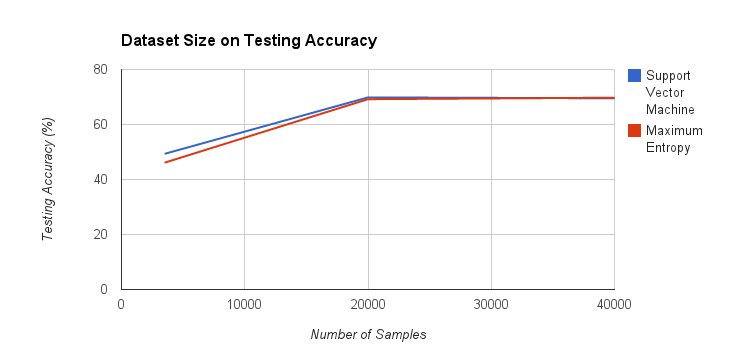
\includegraphics[width=0.7\textwidth]{Dataset_Accuracy.png}
\end{center}
\end{figure}

The size of the dataset noticeably improved the results from 3500 to 20000.  However, after this point it appears that the algorithm converged.  This is seen from the change from 20000 to 40000 samples.  The increase was nearly insignificant for the maximum entropy classifier algorithm.  To summarize, data is able to improve the testing accuracy up to a point, then gains are very small in comparison to early gains.  To further improve the results, either a different classification algorithm would need to be used, or a different set of features would need to be included.  To this end, the following set of experiments will attempt new ways of calculating the feature-vectors for each patent within the \emph{jagged-40000} dataset used in this experiment.

\subsection{Abstract-Bigrams}
For the fourth experiment, the \emph{jagged-40000} dataset was used with \emph{abstract-bigrams} used as the features.  The results indicate that the support vector machine had an accuracy of 72.12\% and the maximum entropy classifier algorithm had an accuracy of 72.57\%.  Overall, this is a slight improvement from experiment 3 of 3\% for the support vector machine and an increase of 3\% for the maximum entropy classifier.

\begin{figure}[!h]
\begin{center}
\caption{SVM with Dimensionality Reduction Testing Accuracy}
\includegraphics[width=0.7\textwidth]{Unigrams_vs_Bigrams.png}
\end{center}
\end{figure}

The small gains from this experiment were strictly due to the use of \emph{abstract-bigram} features.  This is known from the fact that only item which changed between the \emph{jagged-40000} dataset in the previous set of experiments was the move from \emph{description-unigrams} to \emph{abstract-bigrams}.  These results seem to suggest that it is still possible that further gains can be made by creating better features. Therefore, it is still of interest to attempt to create better features while using the largest possible dataset that we have.  The next experiment will attempt this experiment. 

\subsection{tf-idf}
We then used \emph{tf-idf} features on the \emph{jagged-40000} dataset.  The results showed a noticeable improvement from the original dataset, however only a slight improvement from the \emph{abstract-bigrams}.  Specifically, the score for the support vector machine was nearly identical to the \emph{abstract-bigrams}, and the maximum entropy classifier increased by ~5\% from the baseline results.

\begin{figure}[!h]
\begin{center}
\caption{tf-idf for jagged-40000 features}
\begin{tabular}{| r | c | c |}
\hline
\textbf{Features} & \textbf{SVM} & \textbf{Maximum Entropy} \\ \hline
32 & 54.37\% & 66.79\% \\ \hline
100 & 63.62\% & 71.84\% \\ \hline
250 & 72.1\% & 74.15\% \\ \hline
\end{tabular}
\end{center}
\end{figure}

\begin{figure}[!h]
\begin{center}
\caption{tf-idf Features on Testing Accuracy}
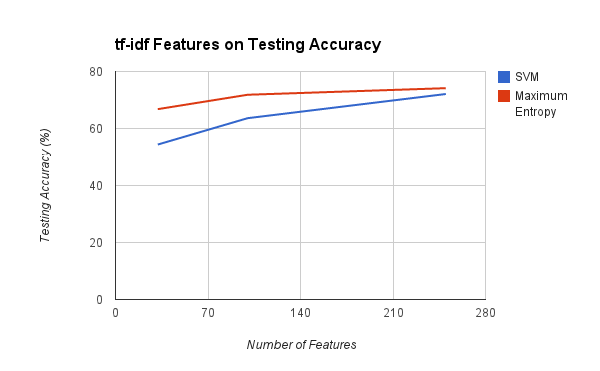
\includegraphics[width=0.7\textwidth]{tfidf.png}
\end{center}
\end{figure}

\emph{tf-idf} is a more abstract set of features that are built off of the \emph{abstract-bigrams}.  The tf-idf features only account for signification information and are therefore better at removing noise from the feature space, and the results of these features were able to further increase the accuracy of the testing algorithm for the maximum entropy classifier.  It is interesting to note, however, that the support vector machine did not gain a boost in accuracy as the maximum entropy classifier did.  Furthermore, the results gained from these features for the maximum entropy classifier were only ~2\%.  These small gains are suggestive that the new features are, in fact, able to improve the results, however the gains are beginning to decline.  It would still be interesting to attempt different features to determine if this trend holds, however, this set of abstract features did perform the best out of all other sets of features we had tested.

\subsection{Summary}

These results have a few interesting findings.  First, dimensionality reduction is able to converge quite early in terms of the dimensionality of the vectors after the process.  This is noted by the maximum entropy classifier converging early in the process, and the laplacian eigenmap for the support vector machine showing early convergence.  
\\A second finding is regarding the sample size used for the patents.  It is interesting to note that the jump from 3500 samples to 20000 samples noticeably improved the algorithm.  However, after that point, the algorithm did not gain in its testing accuracy.  This is suggestive that even when samples are doubled, results will have a tendency to converge.  This is suprising given the fact we had initially expected the results to continue to improve has more data was included.
\\Finally, the last finding of the results are regarding the abstractness of features.  \emph{description-unigrams} did the worst out of all possible sets of features in the construction of feature-vectors.  However, as the features tended to become more abstract in terms of one set of features being built off of an early set, the testing accuracy of the algorithms further improved.  This is noted by the move to \emph{abstract-bigrams} from \emph{description-unigrams} improving the testing accuracy, and furthermore the move from \emph{tf-idf} being built with \emph{abstract-bigrams} have a higher testing accuracy than only the \emph{abstract-bigrams}. Overall, we found these finding to be interesting, and a few of them even surprising.
\section{Classification Evaluation} % (fold)
\label{sec:classification_evaluation}

The IPC classification system was initially created in 1968. Although the subcategories have been changed an expanded since that time, the 8 main top-level categories have not been altered. In the 45 years since the categories were initially established the technological landscape has changed greatly and they may not be as relevant to current and future patent applications. We used several unsupervised techniques and metrics to attempt to evaluate the suitability of the 8 top-level IPC categories.

\ref{tab:skew}Table XXXX shows the proportion of each label class found in \emph{jagged-40000}. We can see that the distribution of patents between the categories is highly skewed, with <ADD CONTENT>. As a first approximation it is desirable that each category occur with roughly equal frequency. Extreme imbalances in the proportions of categories in a sample implies that some are too specific and others are too general. This initial intuition is borne out by metrics of topic coherence that have been used to evaluate the quality of topics generated by unsupervised techniques. We used a coherence metric that compares document frequency with co-document frequency\cite{Mimno_optimizingsemantic}. Specifically, if we define $D(v)$ to be the number of documents in a corpus that contain a given word $v$, $D(v, v')$ to be the number of documents in a corpus that contain both $v$ and $v'$, and $V^{(t)}_M$ to be the $M$ most common words in topic $t$, then we define the coherence of a topic $t$ to be:
\begin{align*}
	C(t;V^{(t)}) = \sum_{m=2}^M \sum_{l=1}^{m-1} \log \frac{D(v^{(t)}_m, v^{(t)}_l)}{D(v^{(t)}_l)}
\end{align*}

This metric is essentially an unnormalized pointwise mutual information, but has been shown to perform better as a coherency metric\cite{Mimno_optimizingsemantic}. Using this metric we calculated coherence scores for each of the IPC classifications in \emph{jagged-40000}\ref{tab:cohere}. We calculated these scores based on the 50 most common words in each. These coherency scores confirm the initial intuition from examining the proportions - that 

\begin{tablehere}
	\label{tab:skew}
	\centering
	\caption{Proportion of IPC classes in \emph{jagged-40000}}
\end{tablehere}

Table of skew


\begin{tablehere}
	\label{tab:cohere}
	\centering
	\caption{coherence scores for IPC classes in \emph{jagged-40000}}
\end{tablehere}

Table of topics


Coherence

In addition to determining how to best classify patents using the CPC labeling scheme, we wanted to evaluate the class system defined by the Patent office.  The patent class system takes it's class structure from the International Patent Classification scheme originated as a result of 1956's European Convention on the International Classification of Patents for Invention in 1968.  Since it's origin, it has been updated in eight editions, the last in 2006.  Despite multiple editions, the top eight categories we examine in this work have not been altered.
  
While the top structure has remained the same, the different types of new technologies are ever changing.  
As many Machine Learning problems have shown previously, tasks which are easy for human's are not easy for machines.  The distinction between a patent in the field of physics and a patent in the field of electricity becomes a difficult problem when the classifier has to rely on only n-grams of terms. 

We observed in our samples that the distribution of incoming patents is shewed.  The proportions of each group in our dataset of patents can be seen in Table Z.  It can be assumed that this distribution can be generalized to the full set of patents.  To investigate how this affects supervised classification, we employed unsupervised methods to generate topics from the dataset of patents.  

 
\subsection{Topic Coherence}
\begin{figure}[!h]
\begin{center}
\caption{Maximum Entropy with Dimensionally Reduction}
\begin{tabular}{|l l|}
\hline

Topic A  &	large updating, establish database,accessible receive,users store,store health,store population,large update,update population,database connected,determines respective,stores health,stores population\\ \hline
Topic B  &	checks brake,predetermined brake,pressure addition,addition checks,checks speed,acceleration dependent,dependent speed,speed dynamic,dynamic cornering,cornering threshold,segments provide,mode recognize,recognize imminent,situation initiate,initiate switch,detecting driving,situation motor,segments operating,mode recognizes,situation initiates\\ \hline	
Topic C  & prismatic face,face InGaN,InGaN base,semiconductor heterostructure,heterostructure median,diameter phosphor,profile inserting,longitudinally cladding,desired collapsing,disposed mixing,refraction gain,core silica,silica doped,amplifier length,length meters,amplifier forming,refraction plurality, refraction inserting, preform drawing, layers collapsing\\ \hline
Topic D  & blend multiple, fibers dimensionally, dimensionally spirally, spirally crimped, crimped selected, consisting cotton, wool silk, silk synthetic, fibers polyamide, polyester polyacrylonitrile, polyacrylonitrile polyethylene, polypropylene polyvinyl, chloride polyvinylidene, chloride polyurethane, fabric stretch, stretch machine, fabric growth, growth greater, greater stretch, terephthalate bicomponent\\\hline
Topic E  & measured flue, period formed, combustion reduced, addition decrease, Disclosed pool, cleaning electric, cavity electrical, vehicle filtering, filtering located, back electrical, located filtering, filtering vehicle, vehicle pulled, pulled pool, pool handle, top drain, bottom allowing, drain completely, completely vehicle, vehicle cavity\\ \hline 
Topic F  & displacement cursor, cursor cost, CI consecutive, consecutive dependent, dependent discrepancy, index speed, speed comprise, comprise keyboard, keyboard entering, entering cost, validating entered, flight display, dedicated page, page displaying, discrepancy fuel, consumption discrepancy, integrated flight, documentation EFB, EFB device, integrated server\\ \hline 
Topic G  & automated measurements, measurements iterative, iterative calculations, calculations controls, routine device, routine software, routine controls, leveling maximum, deviation planarity, planarity nm, nm height, motors instrument, array nanoscopic, tips supported, providing points, determine points, contact tips, interface nanoscopic, nanoscopic tip, tip contacts \\ \hline
Topic H  & signing media, media streams, streams processed, processed accommodate, accommodate resource, requirements environment, application intermediary, intermediary choose, choose advertisement, calculating received, calculated hl, hl equal, authentication calculation, storage streams, authentication obtaining, blocks authentication, authentication apparatus, hash set, calculated equal, block stream \\ \hline
\end{tabular}
\end{center}
\end{figure}

Investigate where things should be split

% section classification_evaluation (end)
\section{Conclusions}
%%%%%%%%%%%%%%%%%%%%%%%%%%%%%%%%%%%%%%%%%%%%%%%%%%%%%%%%%%%%%%%%%%
\section{Conclusions}
\label{sec:Contributions}
%%%%%%%%%%%%%%%%%%%%%%%%%%%%%%%%%%%%%%%%%%%%%%%%%%%%%%%%%%%%%%%%%
%\input{previouswork}


%\begin{multicols}{1}



\bibliography{Sullivan_Cellier_Hobbs}
\bibliographystyle{unsrt}

%\end{multicols}

\end{document}